\chapter{五种感觉}\label{ch:g1:the-five-senses}

闭上眼睛，世界并不会消失：你依然能
听到教室里的声音，闻到午饭的香味，感觉到身下的椅子。
身体有五扇通往世界的“门”——即感觉——每一扇
门都是身体的一个器官，整天为你工作。

\section{五种感觉，五个器官}

\begin{definition}[感觉与感觉器官]\label{def:g1:the-five-senses:sense}
称\emph{感觉}\index{感觉}为身体了解
外部世界的一种方式。每种感觉都通过一个\emph{感觉
器官}\index{感觉器官}来实现，它是身体中专为此工作而构造的部分：
\begin{enumerate}
  \item \emph{视觉}\index{视觉}——\emph{眼睛}\index{眼睛}
        看见光、颜色和形状；
  \item \emph{听觉}\index{听觉}——\emph{耳朵}\index{耳朵}
        听见声音；
  \item \emph{嗅觉}\index{嗅觉}——\emph{鼻子}\index{鼻子}
        闻到气味；
  \item \emph{味觉}\index{味觉}——\emph{舌头}\index{舌头}
        尝到食物的味道；
  \item \emph{触觉}\index{触觉}——\emph{皮肤}\index{皮肤}，
        遍布全身，感觉粗糙与光滑、温暖与寒冷。
\end{enumerate}
\end{definition}

\begin{example}[早餐中的各种感觉]\label{ex:g1:the-five-senses:breakfast}
一碗热巧克力用到了全部五种感觉：眼睛看见蒸汽，
鼻子闻到可可的香味，手上的\omterm{def:g1:the-five-senses:sense}{皮肤}感到碗的温热，
耳朵听见勺子碰碗的声响，舌头——最精彩的部分——
尝到了它的味道。
\end{example}

\begin{omfigure}
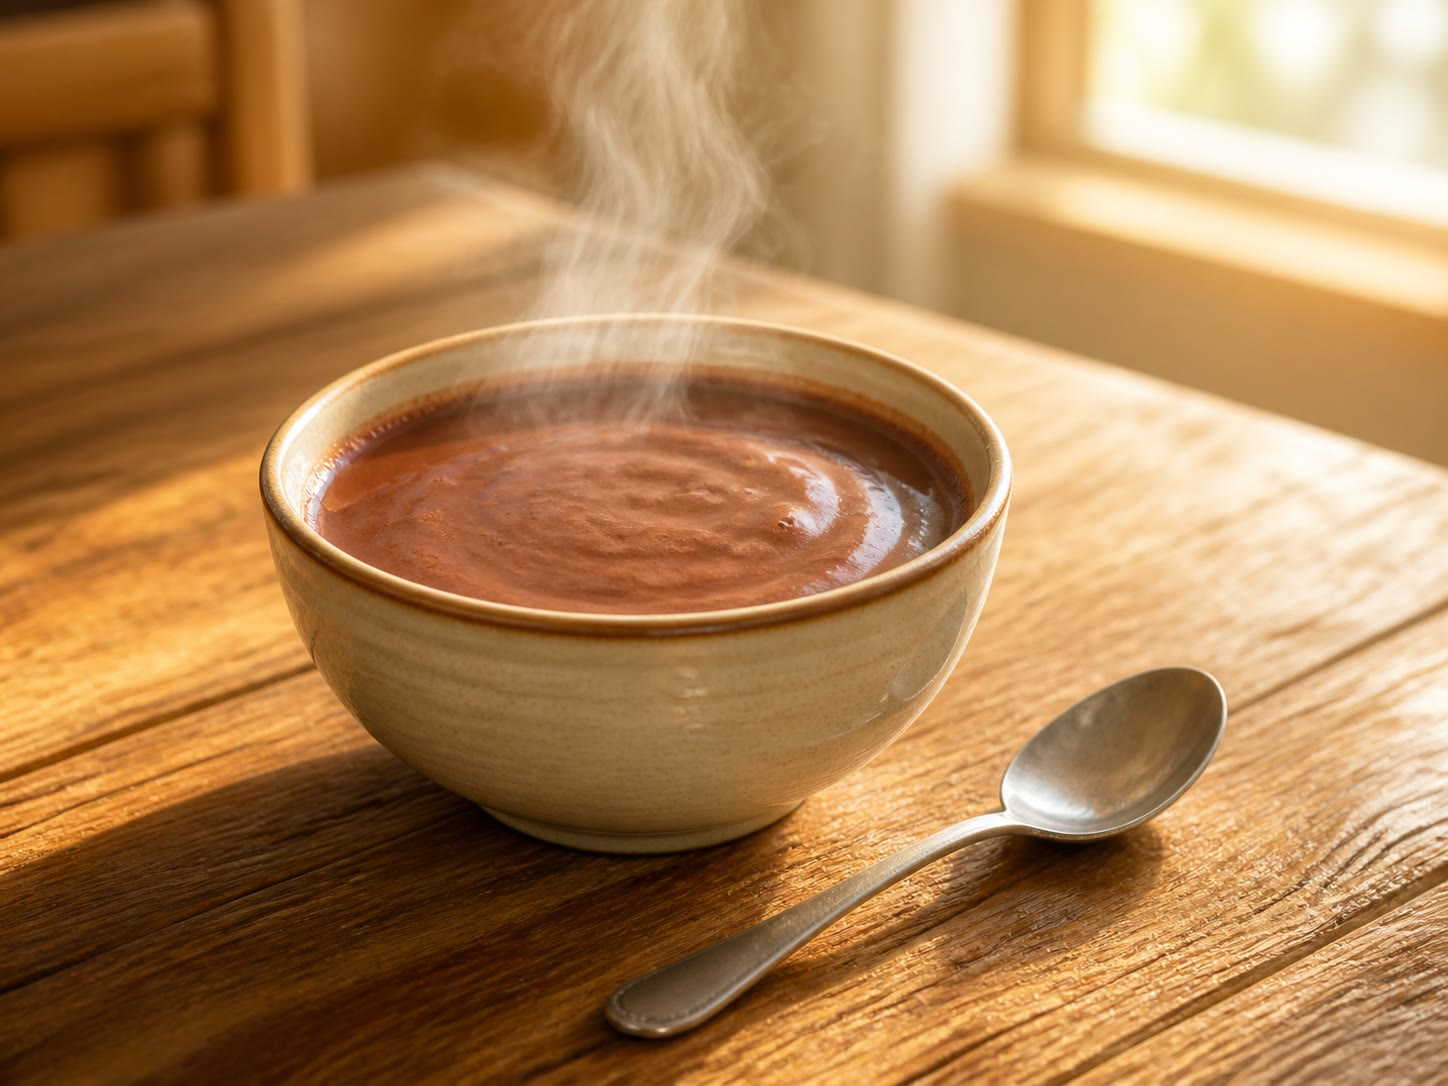
\includegraphics[width=0.58\linewidth]{images/book1/ai/g1-senses-chocolate.jpg}

{\small 一碗热巧克力，在第一口之前
五种感觉已全部投入工作。}
\end{omfigure}

\begin{remark}[触觉无处不在]\label{rem:g1:the-five-senses:skin}
四种\omterm{def:g1:the-five-senses:sense}{感觉器官}位于头部，但触觉器官是
\omterm{def:g1:the-five-senses:sense}{皮肤}，它从头到脚覆盖着你的全身。这就是为什么你能
感觉到\omterm{def:g1:my-body:parts}{脖子}上的微风、鞋子里的小石子和
落在手臂上的瓢虫——这一切都无需用眼睛看。
\end{remark}

\section{感觉向大脑汇报}

\begin{proposition}[送往大脑的信息]\label{prop:g1:the-five-senses:brain}
\omterm{def:g1:the-five-senses:sense}{感觉器官}并不理解它所感受到的东西——它只是\emph{发送
一条信息}。所有信息都在体内传送到
位于头部的\emph{脑}\index{脑}，由它把这些信息综合起来：
“那是奶奶的声音”，“那股气味是烤面包”。没有
脑，眼睛和耳朵就无人可以汇报。
\end{proposition}
\admitted

\begin{omfigure}
\begin{tikzpicture}[scale=0.9]
  % brain box
  \draw[thick, omDef, fill=omDef!8, rounded corners=6pt]
    (4.6,0.2) rectangle (8.2,2.0);
  \node[font=\small\bfseries, omDef] at (6.4,1.55) {脑};
  \node[font=\small, align=center, text width=3.2cm] at (6.4,0.85)
    {把信息 \\整合起来};
  % organs
  \node[font=\small, left] (eye) at (2.2,2.6) {眼睛看见};
  \node[font=\small, left] (ear) at (2.2,1.7) {耳朵听见};
  \node[font=\small, left] (nose) at (2.2,0.8) {鼻子闻到};
  \node[font=\small, left] (skin) at (2.2,-0.1) {皮肤感觉到};
  % arrows
  \draw[->, thick, omMeth] (2.35,2.55) -- (4.55,1.75);
  \draw[->, thick, omMeth] (2.35,1.68) -- (4.55,1.35);
  \draw[->, thick, omMeth] (2.35,0.82) -- (4.55,0.95);
  \draw[->, thick, omMeth] (2.35,-0.02) -- (4.55,0.55);
  \node[font=\small, omMeth] at (3.4,3.0) {信息};
\end{tikzpicture}

{\small 每个\omterm{def:g1:the-five-senses:sense}{感觉器官}都把自己的信息发送给脑，
由脑综合理解它们。（舌头也会汇报，
只是画面会显得太拥挤。）}
\end{omfigure}

\begin{example}[在黑暗中说出物品]\label{ex:g1:the-five-senses:dark}
朋友在你闭着眼睛时，把一件熟悉的物体放进你手里：
钥匙、海绵或勺子。你几乎立刻就能叫出它的名字。
\omterm{def:g1:the-five-senses:sense}{皮肤}发来信息——冰凉、坚硬、有棱角——而脑
回答：“是钥匙”。感觉负责收集，脑负责理解。
\end{example}

\begin{remark}[相互帮助]\label{rem:g1:the-five-senses:together}
各种感觉像一个团队那样协同工作。感冒堵住鼻子时，食物
“尝起来”就会变得寡淡，因为嗅觉承担了风味感受的一半。
当某种感觉完全无法工作时，其他感觉就会学着多做一些：
看不见的人用指尖阅读，靠触觉
认字；过马路时则用耳朵听辨车声。
\end{remark}

\section{保护感觉器官}

\begin{proposition}[脆弱的门]\label{prop:g1:the-five-senses:fragile}
\omterm{def:g1:the-five-senses:sense}{感觉器官}非常宝贵，也很容易受伤。声音太大会伤害
耳朵；直视太阳会伤害眼睛；太烫的一勺
食物会烫伤舌头。受伤的\omterm{def:g1:the-five-senses:sense}{感觉器官}可能长期受损——
所以要保护它们。
\end{proposition}
\admitted

\begin{method}[保护我的感觉器官]\label{met:g1:the-five-senses:protect}
\begin{enumerate}
  \item 不要直视太阳，哪怕只是一瞬间；
  \item 声音要轻柔：不要对着耳朵大喊，戴耳机时
        音量要小；
  \item 不要把任何东西塞进耳朵或鼻子；
  \item 尝之前先把热食吹一吹；
  \item 在光线充足的地方看书、画画。
\end{enumerate}
\end{method}

\begin{example}[隔壁的音乐会]\label{ex:g1:the-five-senses:loud}
声音非常大的音乐过后，耳朵有时会嗡嗡作响一阵子。这种
嗡嗡声，是耳朵在说：“太响了！”。在嘈杂机器旁工作的人
正是出于这个原因才戴上护耳罩——他们的
耳朵要用一辈子。
\end{example}

\section{练习}

\begin{exercise}[$\star$]\label{exo:g1:the-five-senses:1}
说出五种感觉，并分别说出每种感觉对应的\omterm{def:g1:the-five-senses:sense}{感觉器官}。
\end{exercise}

\begin{exercise}[$\star$]\label{exo:g1:the-five-senses:2}
哪种\omterm{def:g1:the-five-senses:sense}{感觉器官}负责感知：（a）气球的颜色？（b）
毯子的柔软程度？（c）雨的气味？（d）铃
声？
\end{exercise}

\begin{exercise}[$\star$]\label{exo:g1:the-five-senses:3}
哪种\omterm{def:g1:the-five-senses:sense}{感觉器官}不在头部？它分布到身体的哪些部位？
\end{exercise}

\begin{exercise}[$\star$]\label{exo:g1:the-five-senses:4}
在\cref{ex:g1:the-five-senses:dark}中，眼睛是闭着的。哪个
器官传递了信息，身体的哪个部分理解了这些信息？
\end{exercise}

\begin{exercise}[$\star$]\label{exo:g1:the-five-senses:5}
患感冒、鼻子堵塞时，食物似乎失去了味道。
吃东西时，通常哪两种感觉会一起发挥作用？
\end{exercise}

\begin{exercise}[$\star$]\label{exo:g1:the-five-senses:6}
写出\cref{met:g1:the-five-senses:protect}中的三条规则，
并说出每条规则保护的是哪种\omterm{def:g1:the-five-senses:sense}{感觉器官}。
\end{exercise}

\begin{exercise}[$\star$]\label{exo:g1:the-five-senses:7}
为什么在噪声很大的机器旁工作的人要戴护耳罩？请用
\cref{prop:g1:the-five-senses:fragile}作答。
\end{exercise}

\begin{exercise}[$\star$]\label{exo:g1:the-five-senses:8}
试一试：闭上眼睛，请一位同伴把三种食物放在你的
鼻子下面——也许是香蕉、奶酪、橘子。不靠眼睛帮忙，你的鼻子
能正确说出几种？
\end{exercise}

\begin{exercise}[$\star\star$]\label{exo:g1:the-five-senses:9}
一位朋友说：“眼睛能理解它所看到的东西。”请改正
这句话，并用\cref{prop:g1:the-five-senses:brain}作依据：
眼睛实际上做了什么？理解又是谁完成的？
\end{exercise}

\begin{exercise}[$\star\star$]\label{exo:g1:the-five-senses:10}
看不见的人如何“阅读”书本，并安全地
过马路？请说明哪些感觉分别承担了哪些工作。
\end{exercise}
